\documentclass[12pt]{article}
\usepackage{amsthm,amssymb,amsfonts,amsmath,amstext,systeme,graphicx,float,tabularx}
\marginparwidth 0pt
\oddsidemargin -1.2 truecm
\evensidemargin  0pt 
\marginparsep 0pt
\topmargin -2.2truecm
\linespread{1}
\textheight 25.8 truecm
\textwidth 18.5 truecm
\newenvironment{remark}{\noindent{\bf Remark }}{\vspace{0mm}}
\newenvironment{remarks}{\noindent{\bf Remarks }}{\vspace{0mm}}
\newenvironment{question}{\noindent{\bf Question }}{\vspace{0mm}}
\newenvironment{questions}{\noindent{\bf Questions }}{\vspace{0mm}}
\newenvironment{note}{\noindent{\bf Note }}{\vspace{0mm}}
\newenvironment{summary}{\noindent{\bf Summary }}{\vspace{0mm}}
\newenvironment{back}{\noindent{\bf Background}}{\vspace{0mm}}
\newenvironment{conclude}{\noindent{\bf Conclusion}}{\vspace{0mm}}
\newenvironment{concludes}{\noindent{\bf Conclusions}}{\vspace{0mm}}
\newenvironment{dill}{\noindent{\bf Description of Dill's model}}{\vspace{0mm}}
\newenvironment{maths}{\noindent{\bf Mathematics needed}}{\vspace{0mm}}
\newenvironment{inst}{\noindent{\bf Instructions}}{\vspace{0mm}}
\newenvironment{notes}{\noindent{\bf Notes }}{\vspace{0mm}}
\newenvironment{theorem}{\noindent{\bf Theorem }}{\vspace{0mm}}
\newenvironment{example}{\noindent{\bf Example }}{\vspace{0mm}}
\newenvironment{examples}{\noindent{\bf Examples }}{\vspace{0mm}}
\newenvironment{topics}{\noindent{\bf Topics}}{\vspace{0mm}}
\newenvironment{outcomes}{\noindent{\bf Expected Learning Outcomes}}{\vspace{0mm}}
\newenvironment{lemma}{\noindent{\bf Lemma }}{\vspace{0mm}}
\newenvironment{solution}{\noindent{\it Solution}}{\vspace{2mm}}
\newcommand{\ds}{\displaystyle}
\newcommand{\un}{\underline}
\newcommand{\bs}{\boldsymbol}

\begin{document}

\baselineskip 18 pt
\begin{center}
	{\large \bf Past paper}
\end{center}
\vspace{0.05cm}
\begin{enumerate}
	\item \textbf{HKDSE Math M2 Sample Paper Q9}\\
	Let $\overrightarrow{OA} = 4\textbf{i} +3 \textbf{j}$, $\overrightarrow{OB} = 3 \textbf{j} +\textbf {k}$ and $\overrightarrow{OC} = 3\textbf{i} + \textbf{j} +5\textbf {k}$. Figure 2 shows the parallelepiped $OADBECFG$ formed by $\overrightarrow{OA}$, $\overrightarrow{OB}$ and $\overrightarrow{OC}$. 
	\begin{figure}[H]
		\centering
		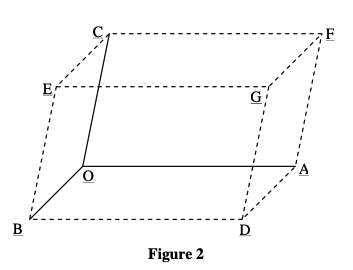
\includegraphics[width = .4\linewidth]{SPFigure2}
	\end{figure}
	\begin{enumerate}
		\item [(a)]Find the area of the parallelogram $OADB$.  
		\item [(b)]Find the volume of the parallelepiped $OADBECFG$.
		\item [(c)]If $C'$ is a point different from $C$ such that the volume of the parallelepiped formed by $\overrightarrow{OA}$, $\overrightarrow{OB}$ and $\overrightarrow{OC'}$ is the same as that of $OADBECFG$, find a possible vector of $\overrightarrow{OC'}$.
	\end{enumerate}
	(6 marks)

	\newpage
	
	\item \textbf{HKDSE Math M2 Sample Paper Q14}\\
	In Figure 3, $\triangle ABC$ is an acute-angled triangle, where $O$ and $H$ are the circumcentre and orthocentre respectively. Let $\overrightarrow{OA} = \textbf{a}$, $\overrightarrow{OB} = \textbf{b}$, $\overrightarrow{OC} = \textbf{c}$ and $\overrightarrow{OH} = \textbf{h}$.
	\begin{figure}[H]
		\centering
		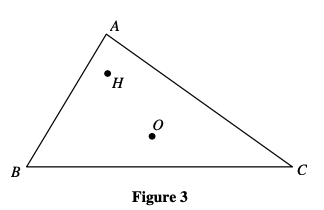
\includegraphics[width = .4\linewidth]{SPFigure3}
	\end{figure}
	\begin{enumerate}
		\item [(a)]Show that $$(\textbf{h} - \textbf{a})//(\textbf{b}+\textbf{c}).$$ \\(3 marks)
		\item [(b)]Let $\textbf{h} - \textbf{a} = t(\textbf{b}+\textbf{c})$, where $t$ is a non-zero constant.\\
		Show that 
		\begin{enumerate}
			\item [(i)]$t(\textbf{b}+\textbf{c}) + \textbf{a} - \textbf{b} = s(\textbf{c}+\textbf{a})$ for some scalar $s$, 
			\item [(ii)]$(t-1)(\textbf{b}-\textbf{a})\cdot (\textbf{c}-\textbf{a}) = 0$.
		\end{enumerate}
		(5 marks)
		\item[(c)]Express $\textbf{h}$ in terms of $\textbf{a}$, $\textbf{b}$ and $\textbf{c}$. \\(2 marks)
	\end{enumerate}

	\item \textbf{HKDSE Math M2 Practice Paper Q12}\\
	Let $\overrightarrow{OA} = \textbf{i}$, $\overrightarrow{OB} = \textbf{j}$ and $\overrightarrow{OC} = \textbf{i} + \textbf{j} + \textbf{k}$ (see Figure 2). Let $M$ and $N$ be points on the straight lines $AB$ and $OC$ respectively such that $AM:MB = a:(1-a)$ and $ON:NC = b:(1-b)$, where $0 < a < 1$ and $0 < b < 1$. Suppose that $MN$ is perpendicular to both $AB$ and $OC$.
	\begin{figure}[H]
		\centering
		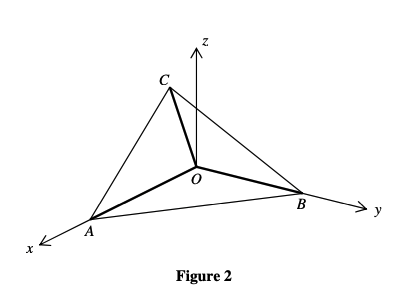
\includegraphics[width = .5\linewidth]{PPFigure2}
	\end{figure}
	\begin{enumerate}
		\item [(a)]
		\begin{enumerate}
			\item [(i)]Show that $$\overrightarrow{MN} = (a+b-1)\textbf{i} +(b-a) \textbf{j} +b \textbf{k}.$$
			\item [(ii)]Find the values of $a$ and $b$.
			\item [(iii)]Find the shortest distance between straight lines $AB$ and $OC$.
		\end{enumerate}
		(8 marks)
		\item [(b)]
		\begin{enumerate}
			\item [(i)]Find $\overrightarrow{AB}\times\overrightarrow{AC}$. 
			\item [(ii)]Let $G$ be the projection of $O$ on the plane $ABC$, find the coordinates of the intersecting point of the two straight lines $OG$ and $MN$.
		\end{enumerate}
		(5 marks)    
  	\end{enumerate}
	
	\newpage
	
	\item \textbf{HKDSE Math M2 2012 Q7}\\
	Figure 3 shows a parallelepiped $OADBECFG$. Let $\overrightarrow{OA} = 6\textbf{i} +2\textbf{j} -\textbf{k}$, $\overrightarrow{OB} = 2\textbf{i} +\textbf{j} $ and $\overrightarrow{OC} = 5\textbf{i} -\textbf{j} +2\textbf{k}$.
	\begin{figure}[H]
		\centering
		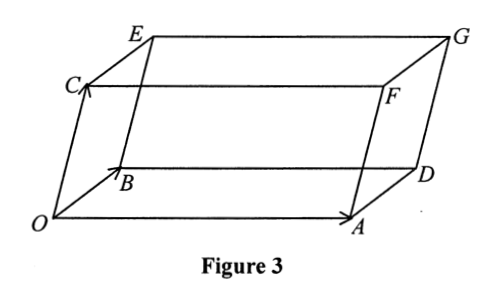
\includegraphics[width = .4\linewidth]{2012Figure3}
	\end{figure}
	\begin{enumerate}
		\item [(a)]Find the area of the parallelogram $OADB$. 
		\item [(b)]Find the distance between point $C$ and the plane $OADB$.
	\end{enumerate}
	(5 marks)

	\item \textbf{HKDSE Math M2 2012 Q12}\\
	Figure 6 shows an acute angled scalene triangle $ABC$, where $D$ is the mid-point of $AB$, $G$ is the centroid and $O$ is the circumcentre. Let $\overrightarrow{OA} = \textbf{a}$, $\overrightarrow{OB} = \textbf{b}$ and $\overrightarrow{OC} = \textbf{c}$.
	\begin{figure}[H]
		\centering
		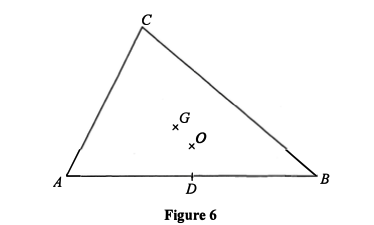
\includegraphics[width = .5\linewidth]{2012Figure6}
	\end{figure}
	\begin{enumerate}
		\item [(a)]Express $\overrightarrow{AG}$ in terms of $\textbf{a}$, $\textbf{b}$ and $\textbf{c}$.\\(3 marks)
		\item [(b)]It is given that $E$ is a point on $AB$ such that $CE$ is an altitude. Extend $OG$ to meet $CE$ at $F$. 
		\begin{enumerate}
			\item [(i)]Prove that $\triangle DOG \sim \triangle CFG$. \\
			Hence find $FG:GO$. 
			\item [(ii)]Show that $\overrightarrow{AF} = \textbf{b} + \textbf{c}$. \\
			Hence prove that $F$ is the orthocentre of $\triangle ABC$.
		\end{enumerate}
		(9 marks)
	\end{enumerate}
	
	\newpage
	
	\item \textbf{HKDSE Math M2 2013 Q10}\\
	Let $\overrightarrow{OA} = 2\textbf{i}$ and 
	$\overrightarrow{OB} = \textbf{i} +2 \textbf{j}$. $M$ is the mid-point of $OA$ and $N$ lies on $AB$ such that $BN : NA = k: 1$. $BM$ intersects $ON$ at $P$ (see Figure 2).
	\begin{figure}[H]
		\centering
		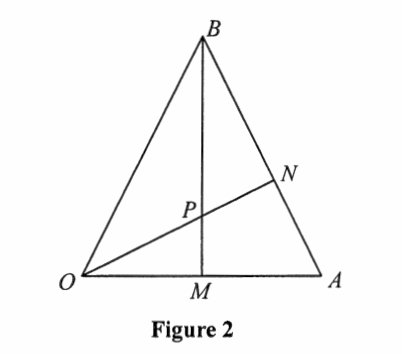
\includegraphics[width = .5\linewidth]{2013Figure2}
	\end{figure}
	\begin{enumerate}
		\item [(a)]Express $\overrightarrow{ON}$ in terms of $k$.
		\item [(b)]If $A$, $N$, $P$ and $M$ are concyclic, find the value of $k$.
	\end{enumerate}
	(5 marks)

	\item \textbf{HKDSE Math M2 2013 Q14}\\
	Figure 5 shows a fixed tetrahedron $OABC$ with $\angle AOB = \angle BOC = \angle COA = 90^{\circ}$. $P$ is a variable point such that $\overrightarrow{AP}\cdot\overrightarrow{BP} + \overrightarrow{BP}\cdot\overrightarrow{CP} + \overrightarrow{CP}\cdot\overrightarrow{AP} = 0$. Let $D$ be the fixed point such that $\overrightarrow{OD} = \displaystyle\frac{\overrightarrow{OA}+\overrightarrow{OB}+\overrightarrow{OC}}{3}$. \\
	Let $\overrightarrow{OA} = \textbf{a}$, $\overrightarrow{OB} = \textbf{b}$, $\overrightarrow{OC} = \textbf{c}$, $\overrightarrow{OP} = \textbf{p}$ and $\overrightarrow{OD} = \textbf{d}$. 
	\begin{figure}[H]
		\centering
		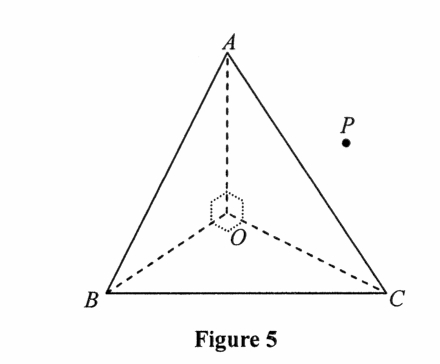
\includegraphics[width = .4\linewidth]{2013Figure5}
	\end{figure}
	\begin{enumerate}
		\item [(a)]
		\begin{enumerate}
			\item [(i)]Show that $\overrightarrow{AP}\cdot\overrightarrow{BP} = \textbf{p}\cdot\textbf{p} - (\textbf{a} + \textbf{b})\cdot\textbf{p}$. 
			\item [(ii)]Using (a)(i), show that $\textbf{p}\cdot\textbf{p} = 2\textbf{p}\cdot\textbf{d}$. 
			\item [(iii)]Show that $|\textbf{p} - \textbf{d}| = |\textbf{d}|$. \\
			Hence show that $P$ lies on the sphere centred at $D$ with fixed radius.
		\end{enumerate}
		(8 marks)
		\item [(b)]
		\begin{enumerate}
			\item [(i)]Alice claims that $O$ lies on the sphere mentioned in (a)(iii). Do you agree? Explain your answer. 
			\item [(ii)]Suppose $P_1$, $P_2$ and $P_3$ are three distinct points on the sphere in (a)(iii) such that $\overrightarrow{DP_1}\times\overrightarrow{DP_2} = \overrightarrow{DP_2}\times\overrightarrow{DP_3}$. Alice claims that the radius of the circle passing through $P_1$, $P_2$ and $P_3$ is $OD$. \\
			Do you agree? Explain your answer.
		\end{enumerate}
		(4 marks)
	\end{enumerate}

	\newpage

	\item \textbf{HKDSE Math M2 2014 Q8}\\
	Let 
	$\overrightarrow{OP} = -\textbf{i} +2 \textbf{j} +2\textbf {k}$, 
	$\overrightarrow{OQ} = \textbf{i} - \textbf{j} +2\textbf {k}$ and 
	$\overrightarrow{OR} = 2\textbf{i} -3 \textbf{j} +6\textbf {k}$. 
	\begin{enumerate}
		\item [(a)]Find $\overrightarrow{OP} \times \overrightarrow{OQ}$. \\
		Hence find the volume of tetrahedron $OPQR$. 
		\item [(b)]Find the acute angle between the plane $OPQ$ and the line $OR$, \\
		correct to the nearest $0.1^\circ$.
	\end{enumerate}
	(8 marks)

	\item \textbf{HKDSE Math M2 2014 Q11}\\
	In Figure 4, $C$ and $D$ are points on $OB$ and $OA$ respectively such that $AD : DO = OC : CB = t : 1-t$, where $0 < t < 1$. $BD$ and $AC$ intersect at $E$ such that $AE : EC = m : 1 $ and $BE : ED = n : 1 $, where $m$ and $n$ are positive. Let $\overrightarrow{OA} = \textbf{a}$ and $\overrightarrow{OB} = \textbf{b}$. 
	\begin{figure}[H]
		\centering
		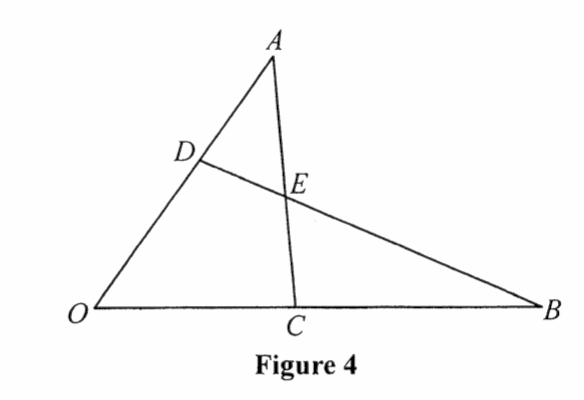
\includegraphics[width = .5\linewidth]{2014Figure4}
	\end{figure}
	\begin{enumerate}
		\item [(a)]
		\begin{enumerate}
			\item [(i)]By considering $\triangle OAC$, express $\overrightarrow{OE}$ in terms of $m$, $t$, $\textbf{a}$ and $\textbf{b}$.
			\item [(ii)]By considering $\triangle OBD$, express $\overrightarrow{OE}$ in terms of $n$, $t$, $\textbf{a}$ and $\textbf{b}$.
			\item [(iii)]Show that $\displaystyle m = \frac{t}{(1-t)^2}$ and $\displaystyle n = \frac{1-t}{t^2}$. 
			\item [(iv)]Chris claims that 
				$$\text{``if }m = n\text{, then }E\text{ is the centroid of }\triangle OAB\text{.''}$$
				Do you agree? Explain your answer.
		\end{enumerate}
		(9 marks)
		\item [(b)]It is given that $OA = 1$ and $OB = 2$. Francis claims that 
			$$``\text{if }AC\text{ is perpendicular to }OB\text{, then }BD\text{ is always perpendicular to }OA\text{.''}$$
			Do you agree? Explain your answer. \\(4 marks)
	\end{enumerate}

	\item \textbf{HKDSE Math M2 2015 Q10}\\
	$OAB$ is a triangle. $P$ is the mid-point of $OA$. $Q$ is a point lying on $AB$ such that $AQ : QB = 1 : 2$ while $R$ is a point lying on $OB$ such that $OR : RB = 3:1$. $PR$ and $OQ$ intersect at $C$. 
	\begin{enumerate}
		\item [(a)]		
		\begin{enumerate}
			\item [(i)]Let $t$ be a constant such that $PC : CR = t : (1-t)$.\\
				By expressing $\overrightarrow{OQ}$ in terms of $\overrightarrow{OA}$ and $\overrightarrow{OB}$, find the value of $t$. 
			\item [(ii)]Find $CQ:OQ$. 
		\end{enumerate}
		(7 marks)
		\item [(b)]Suppose that $\overrightarrow{OA} = 20\textbf{i} -6 \textbf{j} -12\textbf {k}$, $\overrightarrow{OB} = 16\textbf{i} -16 \textbf{j}$ and $\overrightarrow{OD} = \textbf{i} +3 \textbf{j} -6\textbf {k}$, where $O$ is the origin. Find
		\begin{enumerate}
			\item [(i)]the area of $\triangle OAB$, 
			\item [(ii)]the volume of tetrahedron $ABCD$.
		\end{enumerate}
		(5 marks)
	\end{enumerate}
	
	\newpage

	\item \textbf{HKDSE Math M2 2016 Q12}\\
	Let $\overrightarrow{OA} = 2 \textbf{j} +2\textbf {k}$, 
		$\overrightarrow{OB} = 4\textbf{i} + \textbf{j} + \textbf {k}$ and 
		$\overrightarrow{OP} = \textbf{i} +t \textbf{j}$, where $t$ is a constant and $O$ is the origin. It is given that $P$ is equidistant from $A$ and $B$. 
	\begin{enumerate}
		\item [(a)]Find $t$.\\(3 marks)
		\item [(b)]Let $\overrightarrow{OC} = 2 \textbf{i} - \textbf{j} +4\textbf {k}$ and $\overrightarrow{OD} = 3 \textbf{i} +2 \textbf{j} +5\textbf {k}$. Denote the plane which contains $A$, $B$ and $C$ by $\Pi$.
		\begin{enumerate}
			\item [(i)]Find a unit vector which is perpendicular to $\Pi$. 
			\item [(ii)]Find the angle between $CD$ and  $\Pi$. 
			\item [(iii)]It is given that $E$ is a point lying on $\Pi$ such that 
			$\overrightarrow{DE}$ is perpendicular to $\Pi$. Let $F$ be a point such that $\overrightarrow{PF} = \overrightarrow{PA} + \overrightarrow{PB} + \overrightarrow{PC}$. Describe the geometric relationship between $D$, $E$ and $F$. Explain your answer.
		\end{enumerate}
		(10 marks)
	\end{enumerate}

	\item \textbf{HKDSE Math M2 2017 Q3}\\
	$P$ is a point lying on $AB$ such that $AP : PB = 3:2$. Let $\overrightarrow{OA} = \textbf{a}$ and $\overrightarrow{OB} = \textbf{b}$, where $O$ is the origin.
	\begin{enumerate}
		\item [(a)] Express $\overrightarrow{OP} $ in therms of $ \textbf{a}$ and $ \textbf{b}$.
		\item [(b)] It is given that $|\textbf{a}| = 45$, $|\textbf{b}| = 20$ and $\cos{\angle{AOB}} = \displaystyle\frac{1}{4}$. Find
		\begin{enumerate}
			\item [(i)] $\textbf{a}   \cdot  \textbf{b} $, 
			\item [(ii)] $|\overrightarrow{OP}| $. 
		\end{enumerate}
	\end{enumerate}
	(5 marks)

	\item \textbf{HKDSE Math M2 2017 Q10}\\
	$ABC$ is a triangle. $D$ is the mid-point of $AC$. $E$ is a point lying on $BC$ such that $BE : EC = 1 : r$. \\
	$AB$ produced and $DE$ produced meet at the point $F$. It is given that $DE : EF = 1 : 10$. \\
	Let $\overrightarrow{OA} = 2\textbf{i} +3 \textbf{j} -2\textbf {k}$, 
		$\overrightarrow{OB} = 4\textbf{i} +4 \textbf{j} - \textbf {k}$, 
		$\overrightarrow{OC} = 8\textbf{i} -3 \textbf{j} -2\textbf {k}$, where $O$ is the origin.
	\begin{enumerate}
		\item [(a)]By expressing $\overrightarrow{AE}$ and $\overrightarrow{AF}$ in terms of $r$, find $r$.\\(4 marks)
		\item [(b)]
		\begin{enumerate}
			\item [(i)]Find $\overrightarrow{AD} \cdot \overrightarrow{DE}$. 
			\item [(ii)]Are $B, D, C$ and $F$ concyclic? Explain your answer.
		\end{enumerate}
		(5 marks)
		\item[(c)]Let $\overrightarrow{OP} = 3\textbf{i} +10 \textbf{j} -4\textbf {k}$. Denote the circumcentre of $\triangle BCF $ by $ Q$.\\
		Find the volume of the tetrahedron $ABPQ$.\\(3 marks)
	\end{enumerate}

	\item \textbf{HKDSE Math M2 2018 Q12}\\
	The position vectors of the points $A, B, C$ and $D$ are  
	$4\textbf{i} -3 \textbf{j} + \textbf {k}$, 
	$-\textbf{i} +3 \textbf{j} -3 \textbf {k}$, 
	$7\textbf{i} - \textbf{j} +5 \textbf {k}$ and 
	$3\textbf{i} -2 \textbf{j} -5 \textbf {k}$  
	respectively. Denote the plane which contains $A, B$ and $C$ by $\Pi$. Let E be the projection of  $D$ on $\Pi$.
	\begin{enumerate}
		\item [(a)]Find
		\begin{enumerate}
			\item [(i)]$\overrightarrow{AB} \times \overrightarrow{AC}$,
			\item [(ii)]the volume of the tetrahedron $ABCD$,
			\item [(iii)]$\overrightarrow{DE}$.
		\end{enumerate}
		(5 marks)
		\item [(b)]Let $F$ be a point lying on $BC$ such that $DF$ is perpendicular to $BC$.
		\begin{enumerate}
			\item [(i)]Find $\overrightarrow{DF}$. 
			\item [(ii)]Is $\overrightarrow{BC} $ perpendicular to $\overrightarrow{EF}$ ? Explain your answer.
		\end{enumerate}
		(5 marks)
		\item[(c)]Find the angle between $\triangle BCD$ and $\Pi$. \\(3 marks)
	\end{enumerate}
	
	\newpage

	\item \textbf{HKDSE Math M2 2019 Q12}\\
	Let $\overrightarrow{OA} = \textbf{i} -4 \textbf{j}+ 2\textbf {k}$, $\overrightarrow{OB} = -5\textbf{i} -4 \textbf{j} +8\textbf {k}$ and $\overrightarrow{OC} = -5\textbf{i} -12 \textbf{j} +t\textbf {k}$, where $O$ is the origin and $t$ is a constant. It is given that $|\overrightarrow{AC}| = |\overrightarrow{BC}|$. 
	\begin{enumerate}
		\item [(a)]Find $t$. \\(3 marks)
		\item [(b)]Find $\overrightarrow{AB} \times \overrightarrow{AC}$. \\(2 marks)
		\item [(c)]Find the volume of the pyramid $OABC$. \\(2 marks)
		\item [(d)]Denote the plane which contains $A$, $B$ and $C$ by $\Pi$. It is given that $P$, $Q$ and $R$ are points lying on $\Pi$ such that $\overrightarrow{OP} = p\textbf{i}$, $\overrightarrow{OQ} = q\textbf{j}$ and $\overrightarrow{OQ} = r\textbf{k}$. Let $D$ be the projection of $O$ on $\Pi$.
		\begin{enumerate}
			\item [(i)]Prove that $pqr \neq 0$. 
			\item [(ii)]Find $\overrightarrow{OD}$. 
			\item [(ii)]Let $E$ be a point such that $\overrightarrow{OE} = \displaystyle\frac{1}{p}\textbf{i}+\frac{1}{q}\textbf{j}+\frac{1}{r}\textbf{k}$. Describe the geometric relationship between $D$, $E$ and $O$. Explain your answer.
		\end{enumerate}
		(6 marks)
	\end{enumerate}

	\item \textbf{HKDSE Math M2 2020 Q12}\\
	Let $\overrightarrow{OP} = \textbf{i} + \textbf{j}+ 4\textbf {k}$ and $\overrightarrow{OQ} = 5\textbf{i} -7 \textbf{j}- 4\textbf {k}$, where $O$ is the origin. \\
	$R$ is a point lying on $PQ$ such that $PR:RQ = 1:3$. 
	\begin{enumerate}
		\item [(a)]Find $\overrightarrow{OP} \times \overrightarrow{OR}$. \\(2 marks)
		\item [(b)]Define $\overrightarrow{OS} = \overrightarrow{OP} + \overrightarrow{OR}$. Find the area of the quadrilateral $OPSR$. \\(2 marks)
		\item [(c)]Let $N$ be a point such that $\overrightarrow{ON} = \lambda(\overrightarrow{OP}\times \overrightarrow{OR})$, where $\lambda$ is a real number.
		\begin{enumerate}
			\item [(i)]Is $\overrightarrow{NR}$ perpendicular to $\overrightarrow{PQ}$? Explain your answer.
			\item [(ii)]Let $\mu$ be a real number such that $\overrightarrow{NQ}$ is parallel to $11\textbf{i} + \mu\textbf{j}-10\textbf {k}$. 
			\begin{enumerate}
				\item [(1)]Find $\lambda$ and $\mu$. 
				\item [(2)]Denote the angle between $\triangle OPQ$ and $\triangle NPQ$ by $\theta$. Find $\tan{\theta}$.
			\end{enumerate}
		\end{enumerate}
		(8 marks)
	\end{enumerate}

	\item \textbf{HKDSE Math M2 2021 Q12}\\
	The position vectors of the points $A$, $B$, $C$ and $D$ are  $t\textbf{i} +14 \textbf{j}+s \textbf {k}$, $12\textbf{i} -s \textbf{j}-2 \textbf {k}$, $(s+2)\textbf{i} -16 \textbf{j}+10 \textbf {k}$ and $-t\textbf{i} +(s+2) \textbf{j}+14 \textbf {k}$  respectively, where $s$, $t \in \mathbb{R}$. Suppose that $\overrightarrow{AB}$ is parallel to $5\textbf{i} -4 \textbf{j}-2 \textbf {k}$. \\Denote the plane which contains $A$, $B$ and $C$ by $\Pi$.
	\begin{enumerate}
		\item [(a)]Find
		\begin{enumerate}
			\item [(i)]$s$ and $t$,
			\item [(ii)]the area of $\triangle ABC$,
			\item [(iii)]the volume of the tetrahedron $ABCD$,
			\item [(iv)]the shortest distance from $D$ to $\Pi$.
		\end{enumerate}
		(9 marks)
		\item [(b)]Let $E$ be the projection of  $D$ on $\Pi$. Is $E$ the circumcentre of $\triangle ABC$? Explain your answer.\\(4 marks)
	\end{enumerate}
	
	\newpage

	\item \textbf{HKDSE Math M2 2022 Q12}\\
	Consider $\triangle ABC$. Denote the origin by $O$. 
	\begin{enumerate}
		\item [(a)]Let $D$ be a point lying on $BC$ such that $AD$ is the angle bisector of $\angle BAC$. \\
		Define $BC = a$, $AC = b$  and  $AB = c$. 
		\begin{enumerate}
			\item [(i)]Using the fact that $BD:DC = c:b$, prove that $$\overrightarrow{AD} = -\overrightarrow{OA}+\displaystyle\frac{b}{b+c}\overrightarrow{OB} + \displaystyle\frac{c}{b+c}\overrightarrow{OC}.$$
			\item [(ii)]Let $E$ be a point lying on $AC$ such that $BE$ is the angle bisector of $\angle ABC$. \\
			Define $$\overrightarrow{OJ} = \displaystyle\frac{a}{a+b+c}\overrightarrow{OA}+\displaystyle\frac{b}{a+b+c}\overrightarrow{OB}+\displaystyle\frac{c}{a+b+c}\overrightarrow{OC}.$$
				Prove that $J$ lies on $AD$. Hence, deduce that $AD$ and $BE$ intersect at $J$.
		\end{enumerate}
		(7 marks)
		\item [(b)]Suppose that $\overrightarrow{OA} = 35\textbf{i} +9 \textbf{j}+ \textbf {k}$, $\overrightarrow{OB} = 40\textbf{i} -3 \textbf{j}+ \textbf {k}$ and $\overrightarrow{OC} =  -3 \textbf{j}+ \textbf {k}$. Let $I$ be the incentre of $\triangle ABC$. 
		\begin{enumerate}
			\item [(i)] Find $\overrightarrow{OI}$. 
			\item [(ii)] By considering $\overrightarrow{AI} \times \overrightarrow{AB}$, find the radius of the inscribed circle of $\triangle ABC$. 
		\end{enumerate}
		(5 marks)
	\end{enumerate}            

	\item \textbf{HKDSE Math M2 2023 Q10}\\
	Let $O$ be the origin. The position vectors of $P$ and $Q$ are $-2\textbf{i} - \textbf{k}$ and $2\textbf{i} -\textbf{j}+ \textbf{k}$ respectively. Denote the circle passing through $O$, $P$ and $Q$ by $C$. Let $R$ be a point lying on $PQ$ such that $OR$ is perpendicular to $OQ$.
	\begin{enumerate}
		\item [(a)] By considering the ratio of $PR$ to $RQ$, find $\overrightarrow{OR}$. \\(3 marks)
		\item [(b)] $OR$ produced meets $C$ at another point $S$. Find $\overrightarrow{OS}$. \\(3 marks)
		\item [(c)] Let $\Pi$ be the plane which contains $C$.
		\begin{enumerate}
			\item [(i)] Find a non-zero vector which is perpendicular to $\Pi$.
			\item [(ii)] Let $G$ be the center of $C$. Denote the projection of point $A(-6, -22,2)$ on $\Pi$ by $B$. Describe the geometric relationship between $O$, $B$ and $G$. Explain your answer.
		\end{enumerate}
		(6 marks)
	\end{enumerate}

\end{enumerate}





\end{document}